\section{Contextualization}

Documents are at the core of corporate society, and they often hold immeasurable value, representing contracts, employment relationships, loans, and identities. Recently, as technology becomes more accessible, documents have become increasingly more digital, some never being printed on paper. These documents often have all important information already separated in the file's metadata and require no extra intelligence to classify or extract the information. However, many organizations still receive documents in physical form, for example, when dealing directly with individual customers, which makes full digitization impractical in many cases.

In such a scenario, organizations require a document understanding pipeline to validate document types and extract data for business decision-making (see \refFig{fig:compliance}). 
Historically, this process relied on manual human labor.
Following the adoption of \gls{OCR} engines~\cite{kay_tesseract_2007, mindee_doctr_2021}, tasks shifted from manual data entry to back-office analysis, where human operators verified compliance and classified documents.
However, given the scale of modern data, manual processing has become computationally and economically inefficient.
Today, with the current technologies, especially with the advancement of \glspl{NN} and the cheapening of computing systems, automated pipelines have replaced many manual workflows in many companies. 
Given this context, this work addresses the challenge of automatic document classification.

\begin{figure}[htbp]
%\isPreprints{\centering}{} % Only used for preprints
\centering
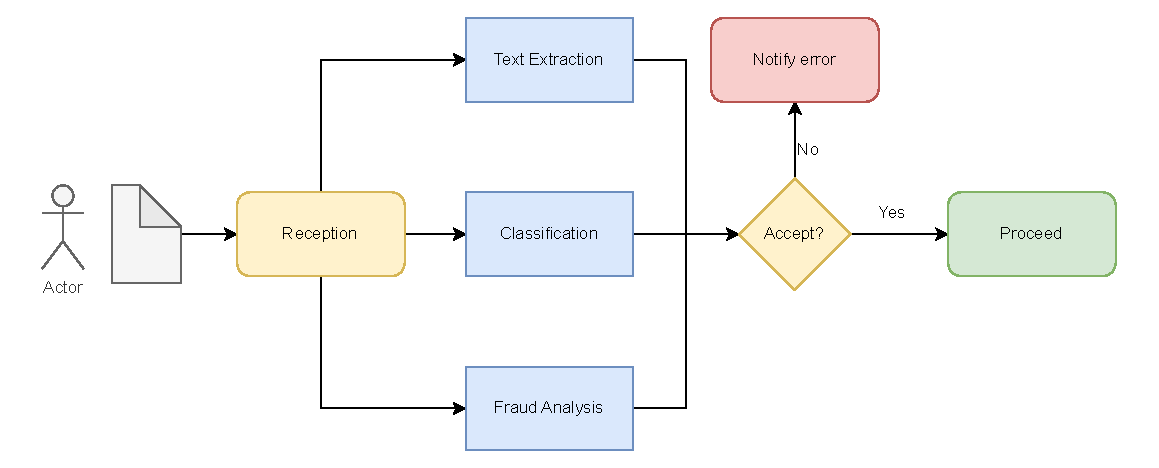
\includegraphics[width=1\linewidth]{images/diagrama-compliance.drawio.pdf}
\caption{Simplified view of a document compliance pipeline. In this diagram, text extraction, document classification and fraud analysis are being used together to decide upon the acceptance of the received document.}
\label{fig:compliance}
\end{figure}


% \red{DIAGRAMA ZSL VS TRADICIONAL AQUI}

\section{Problem Description}
\label{sec:problem}


Document Classification is defined by the categorization of documents into predefined classes~\cite{liu_document_2021}.
\acrfull{DIC} is a specialized subset of this task where textual data is not natively available, as inputs often consists of photos or scans of physical documents.
Consequently, textual analysis in \gls{DIC} requires an initial extraction step using \gls{OCR} algorithms.
While \gls{AI} and \acrfull{DL} can automate classification using image-only architectures, which reduces computational overhead by bypassing \gls{OCR}, visual features alone may be insufficient for certain tasks.
In such cases, models may utilize textual features or employ multimodal fusion techniques.
This problem is already known and well studied.
For instance, Bakkali et al.~\cite{bakkali_eaml_2021} achieved $97.70\%$ accuracy on the \gls{RVL-CDIP}~\cite{harley_evaluation_2015}, a popular \gls{DIC} dataset.

The problem arises when previously accepted documents change in form or when entirely new document classes, not previously considered, must be handled and categorized. In such cases, models are typically retrained, as traditional classification networks may struggle to generalize to new document layouts or entirely new classes. Traditional \gls{DL} classification methods require a predefined set of labels and cannot output a label outside the original training set. Therefore, introducing new labels to the model means retraining the model, changing the output layer into a wider one with more options. Very often, this also means weeks or months of data engineering, labeling, and model training. The alternative is to use \acrfull{ZSL} techniques, which allow models to generalize to classes that were not seen during training~\cite{xian_zero-shot_2019}.


This work focuses on the \gls{ZSL} on \gls{DIC}, where the model must correctly classify a document image class that was not in the training set and therefore previously unseen by the model. \blue{\gls{ZSL} techniques enable models to be considerably more flexible}, as they are not limited by the classes used in training. Most \gls{ZSL} systems work by semantically mapping embeddings into a feature space, where \blue{embeddings} from the same class are all clustered together, and different classes are placed far apart. \blue{This is called metric learning, where the model is optimized to map the training samples in regards to a given metric (e.g. euclidean distance)}. Developing a robust \gls{ZSL} system requires identifying a set of features that serve as discriminative representations, ensuring that document proximity in the feature space correlates strictly with class membership. Using a \gls{DL} approach, this could also demand a dataset with a wide variety of classes, enough so that the model learns what makes two documents similar or different. These conditions allow \gls{ZSL} models to group together documents, even if them were entirely novel document types.


However, not all classification datasets are suitable for effective \gls{ZSL} applications.
The scarcity of specialized datasets remains a primary obstacle in document-image \gls{ZSL}, leading to a lack of standardized methodologies.
As consequence, other main challenge is the lack of a state-of-the-art methodology.
Due to the challenge in achieving \gls{ZSL} classification with the currently available datasets, researchers often employ diverse approaches that yield incomparable results \cite{sinha_cica_2024}, contrasting with the established frameworks and baselines found in traditional classification and information extraction.
Recent approaches have used pretrained \glspl{LLM}~\cite{scius-bertrand_zero-shot_2025} to achieve \gls{ZSL} by exploiting the models' previous knowledge. However, since it often requires a fine-tuning step, the potential cost-efficiency of this strategy may be reduced.

% \red{(Acredito que a banca vai reclamar disso aqui e pedir uma justificativa referenciada para explicar porque o fine-tuning limita o useo das LLMs)}. 
% O fine-tuning não limita as LLMs, mas o fato de ter fine-tuning implica que usar o modelo vai ser mais custoso. Vou tentar reescrever pra deixar mais claro

\section{\blue{Research Objectives}}
\label{sec:objectives}

The primary goal of this research is to develop a complete \gls{ZSL} framework for \gls{DIC}, that is, a classification model that does not require retraining every time a new class of document is introduced. To achieve this, this work pursues the following specific goals:
\begin{enumerate}
    \item Design and curate a specialized dataset for zero-shot document image classification, ensuring proper class separation between training and testing sets;
    \item Develop a framework using metric learning techniques to enable document classification based on visual similarity;
    \item Evaluate and compare different \gls{NN} backbones within the proposed framework to establish performance benchmarks;
\end{enumerate}

\subsection{\blue{Research Hypothesis}}

This work is grounded on the following hypothesis:
\begin{quote}
\textit{Document images that share similar visual layouts contain discriminative features that can be learned through metric learning, enabling accurate classification of previously unseen document classes by measuring visual similarity, without requiring class-specific training.}
\end{quote}
This hypothesis is supported by the premise that document layouts within the same class exhibit consistent visual patterns (placement of text blocks, logos, signatures, etc.) that distinguish them from other classes, and that these patterns can be captured through vision models trained with a metric learning framework.

\section{Research Contributions}

The proposed framework measures the similarity between documents to determine if they belong to the same category, regardless of whether that class was present during training. Specifically, our \acrfull{VDM} method formulates zero-shot classification as a binary matching problem, wherein the system determines if pairs of documents have visual correspondence (i.e., if they match visually or not).

This work makes several key contributions:
\begin{enumerate}
    \item Introduces a novel document image dataset specifically designed for the task of document \gls{ZSL} classification, enabling the development and evaluation of models in this domain.
    \item Proposes the \gls{VDM} approach, which is based on image similarity and leverages \gls{ZSL} techniques to enable generalization across unseen document layouts without requiring additional intervention on the model itself.
    \item Delivers a systematic evaluation of well established backbones in the context of zero-shot document layout matching, offering valuable benchmarks for future research.
\end{enumerate}

This research resulted in two publications. The first, titled \textit{Towards Zero-Shot Document Image Classification}~\cite{11223349}, was published at SIBGRAPI in Salvador, Brazil, and introduces the \gls{VDM} solution and the method to use it with the novel \gls{LA-CDIP} dataset. The second publication, titled \textit{Visual Document Matching for Zero-Shot Document Classification}~\cite{10.1007/978-3-032-09368-4_12}, was published at ICDAR in Wuhan, China, and extends the first work by comparing the results with the performance of Large Language Models. At the same time, the solution is currently implemented in one of the biggest banks in Brazil, having categorized in real time millions of documents into their respective classes, as soon as they are sent by the users.

\section{About this work}

This \blue{work} is structured as follows: \refCap{2-Teorica} establishes the theoretical foundation, while \refCap{3-TrabalhosRelacionados} reviews the state of the art in \gls{ZSL} and visually-rich document understanding, highlighting existing methods and their limitations. \refCap{4-SolucaoProposta} introduces the proposed \gls{VDM} framework, detailing its architecture and components. \refCap{5-Metodologia} presents the data-labeling process and the experimental setup. \refCap{6-Resultados} describes the experimental setup, datasets, evaluation metrics, and baseline comparisons, followed by a comprehensive analysis of the results. Finally, \refCap{7-Conclusao} concludes the \blue{work} by summarizing the key contributions, discussing potential applications, and outlining directions for future research.

